%!TEX root = ../BGP_for_networks_who_peer.tex
\chapter{BGP Communities}
\label{ch:BGP Communities}
\section{Introduction}
In the last chapter, we learned about a number of BGP attributes. This chapter is now about a single attribute called ``BGP community''. Why a whole chapter about one attribute?

BGP communities are very important if you build your network for multiple peerings and multiple upstreams. They help you to keep your BGP infrastructure scalable and assist you in implementing your routing policy.

BGP communities were not a part of BGP from the beginning. They were introduced in 1996 in \cite{rfc1997}. This is a great example of how BGP got extended when needed: BGP was designed with future enhancement in mind. Two BGP speaking routers can still ``talk'' to each other, even if both do not have the same feature-set. When setting up a BGP session, both announce what features they support and if an optional feature marked as ``optional'' is not supported by both sides, a session still comes up.

So what are BGP communities? They are like a sticker on your suitcase. You can add information to a BGP prefix announcement with them, but they only have the meaning you define. In themselves, they are nothing more than a number stuck on your announcement. Some BGP communities have a pre-defined meaning; we call them ``well-known communities''. Their meanings are defined in \glspl{rfc}.

\section{Original communities}
What we now call ``original'' BGP communities were introduced in 1996 in \cite{rfc1997}. An original BGP community attribute is just a 32-bit number, attached as an optional attribute to a BGP prefix announcement. You can attach as many communities as you want (within reason). The community attribute was defined as optional (does not have to exist) and transitive (is kept when re-announcing the prefix).

Some number ranges were defined as reserved: 0x00000000-0x0000ffff, 0xffff0000-0xffffffff. In these reserved ranges, a number of ``well-known'' communities were defined (see \ref{wellknown}).

Although ``just a 32-bit number'' it was also defined that the first half should encode an AS number (Autonomous System Numbers were only 16bit in these days). To make reading easier, the notation of communities in routers and documentation was later defined as two 16-bit numbers separated by a colon (like 6695:1200).

The purpose of communities was (and still is) to add a property to prefixes - the ``translation'' between the numerical value and its meaning should be up to the party defining the community.

\section{Extended communities}
With the arrival of 32bit AS-Numbers, it was no longer possible to encode the community-defining AS number in the first half. So in 2006 \emph{extended communities} were defined in \cite{rfc4360}.

Unfortunately, the authors of the RFC did not only want to solve the 32bit problem but added also a number of other features:
\begin{itemize}
  \item A 16-bit type field allowing different community types.
  \item A ``transitive'' bit as part of this field to define if a type was transitive (should be forwarded between ASes) or not.
  \item An IANA-bit, noting if a type was IANA-assigned or experimental.
\end{itemize}
The initial \cite{rfc4360} still deals with only 16-bit AS numbers, only in \cite{rfc5668} it is finally defined to have a 32-bit AS number as ``global administrator'' in an extended community. As 16 bits are already used for the type field, that leaves only 16 bit as an argument or value field.

Extended communities were never really liked by the operators - too confusing and over-engineered. So another type of community was needed.

\section{Large communities}
``Large communities'' fix the shortcomings of extended communities. Defined in \cite{rfc8092}, they go back to the simplistic approach of the original communities: Three simple 32-bit values. The first 32-bit number is defined as the ``Global Administrator'' - an AS number (32bit!) giving meaning to the two remaining numbers. These two can be seen as simply two values or as one function number plus one numerical parameter.

The notation is three numbers separated by colons (``:''). As large communities are kind of new (defined in 2017), you need quite recent software versions for your router. Implementation status is being tracked at \url{http://largebgpcommunities.net/implementations/}, there you also can see the minimum sofware you need for most implementations.

Mind that \emph{Juniper} routers notate large communities like ``large:global administrator:value1:value2'' - so you have to prefix them with ``large:'' otherwise the router reports a syntax error.

Figure \ref{fig:communities} shows all three community types.

\begin{figure}
  \centering
  \includegraphics[width=\linewidth,page=5]{img/Drawings.pdf}
  \caption{Original, Extended, and Large BGP Communities}
  \label{fig:communities}
\end{figure}


\section{Some well-known communities}
\label{wellknown}
So-called well-known communities are defined in RFCs and must be processed by all BGP speaking entities. The following four well-known communities are quite useful.

\subsection{NO-EXPORT}
BGP prefixes tagged with \emph{NO-EXPORT} must not be advertised via eBGP to other Autonomous Systems. Defined in \cite{rfc1997}, this well-known community is useful for:
\begin{itemize}
  \item Announcing \emph{more specific} prefixes to your eBGP neighbors and making sure they are not announced further. To do this, set NO-EXPORT on your outgoing route-map (or similar).
  \item Keeping your own specific routes inside your own AS. For this, set NO-EXPORT when injecting your prefixes into BGP and leave it off the network blocks which should be announced externally.
\end{itemize}

\subsection{NO-ADVERTISE}
This well-known community is even stricter then NO-EXPORT. \emph{NO-ADVERTISE} forbids a router from announcing a prefix to any BGP neighbor; this also includes iBGP.

\subsection{BLACKHOLE}
Defined 2016 in \rfc{7999}, this well-known community asks the receiving operator to blackhole or block all traffic destined to the prefix with this community attached.

For this to work properly, the receiver should accept longer than usual prefixes (up to /32 in IPv4 and up to /128 in IPv6). Also, the receiver should not propagate these prefixes further, so either the sender also attaches a NO-EXPORT or the receiver should.

The purpose, of course, is to fight DOS or DDOS attacks.

\subsection{ANYCAST}
Not yet an RFC, this community is for tagging \emph{anycast} routes. There is no default processing of the community - it is up to an operator to define what to do with so tagged routes. 

\section{Examples}
\subsection{Setting communities when receiving}
Set a community when receiving prefixes from the outside. The community should be added to the existing communities.

\subsubsection{Cisco}
\begin{verbatim}
route-map customer-in permit 200
  set community 64500:47000 additive
\end{verbatim}
The ``additive'' keyword ensures that the community is added to the list of already existing communities.

\subsubsection{FRRouting}
Same syntax as Cisco.

\subsubsection{Mikrotik}
Instead of route-maps, Mikrotik has filters. Please check the documentation for details.
\begin{verbatim}
  /routing filter
  add chain=customer-in append-bgp-communities=64500:47000
\end{verbatim}
Using the ``append-bgp-communities'' keyword appends the community to the list of already attached communities. To clear the community list first, use ``set-bgp-communities''.

\subsection{Setting communities when redistributing}
In this case, we do not receive the prefixes via eBGP, but we distribute our own network blocks.

\subsubsection{Cisco}
\begin{verbatim}
  router bgp 64500
    redistribute static route-map static-to-bgp
  !
  route-map static-to-bgp permit 100
    set community 64500:41000
\end{verbatim}
Note that the ``additive'' keyword is missing here; usually, this would remove all existing communities. But as we inject new prefixes into BGP, there are no communities set yet.

\subsubsection{FRRouting}
Same syntax as Cisco.

\subsubsection{Mikrotik}
Communities can be added directly to static routes, which are then redistributed:
\begin{verbatim}
  /routing  bgp instance
  set redistribute-static=yes

  /ip route
  add dst-address=198.51.100.0/24 gateway=loopback0 bgp-communities=64500:41000
\end{verbatim}


\subsection{Removing communities}
Removing communities can be done either by removing all communities, specific ones, or ones matching certain criteria. All three cases will be shown.

\subsubsection{Cisco}
Delete one community (or more than one, explicitly listed):
\begin{verbatim}
  ip community-list standard delete-list permit 64500:10000
  !
  route-map customer-in permit 100
    set comm-list delete-list delete
\end{verbatim}
You can add more communities to \emph{delete-list} but with a standard list in Cisco, you have to explicitly list all you want to have deleted.

With an expanded list, you can delete communities based on a pattern:
\begin{verbatim}
  ip community-list expanded delete-pattern permit 64500:1[0-9][0-9][0-9][0-9]
  !
  route-map customer-in permit 100
    set comm-list delete-pattern delete
\end{verbatim}
Here we delete all communities with AS64500 in the first part and have 10000-19999 in the 2nd part. The community number is treated as a string and a regular expression is used for matching. For details on how regular expressions are built, please check Cisco documentation.

If you want to delete all communities incoming, you can use the same method:
\begin{verbatim}
  ip community-list expanded delete-all permit .*
  !
  route-map customer-in permit 100
    set comm-list delete-all delete
\end{verbatim}

\subsubsection{FRRouting}
Deleting \emph{all}  communities in FRRouting is easy:
\begin{verbatim}
  route-map customer-in permit 100
    set community none
\end{verbatim}


\subsubsection{Mikrotik}
Mikrotik does not have regular expression matching for communities, nor does it have a delete community command.

\subsection{Scrubbing communities incoming}
In this example, we want to do a more sophisticated check and change.
\begin{itemize}
  \item Customers are allowed to send communities like 64500:4xxxx
  \item Everything else starting with 64500: has to be removed
  \item If they do not send any community starting with 64500:4xxxx, per default 64500:47000 is set
\end{itemize}

\subsubsection{Cisco}
\begin{verbatim}
  ip community-list expanded delete-incoming permit 64500:[0-35-9][0-9]*
  !
  ip community-list expanded command-community permit 64500:4[0-9][0-9][0-9][0-9]
  !
  route-map customer-in permit 100
    continue
    set comm-list delete-incoming delete
  !
  route-map customer-in permit 200
    match community command-community
  !
  route-map customer-in permit 300
    set community 64500:47000 additive
\end{verbatim}
Explanation:
\begin{itemize}
  \item In entry 100, we simply remove what we do not want. The ``continue'' statement makes sure that processing continues even if we have a successful match.
  \item In entry 200, we only check if a command-community has been set by the customer. Because there is no ``continue'' statement, the route-map terminates at success. If no command-community was set, the next entry is processed.
  \item Entry 300 has no match-statement so it always succeeds. A community of 64500:47000 is set and the route-map terminates.
\end{itemize}

\subsubsection{FRRouting}
Same as Cisco IOS.

\subsubsection{Mikrotik}
You cannot do this on Mikrotik. If you allow your customers to set certain communities, you must filter-check for exactly these and either directly apply some action or let them through and remove anything else. Example:
\begin{verbatim}
  /routing filter
  add action=accept bgp-communities=64500:41000 chain=customer-in \
    set-bgp-communities=64500:41000
\end{verbatim}
This matches if community 64500:41000 is set, removes all other communities, and sets 64500:41000 exclusively. Also, processing of the filter chain is terminated. This gives you some basic possibilities, but more complex filters are not possible.

\section{What to do with them?}
Now that we know what communities are and how to add them to prefixes (and remove them) the question remains: What to do with them?

Before they were introduced, rules for filtering and rules for implementing your routing policy had to be configured on every device. Communities now give you  the possibility that you can tag prefixes with a specific community once  you receive them, and act later depending on that community.

If we go back to the ``sticker on a suitcase'' comparison, we can distinguish between two types of communities:
\begin{description}
  \item[Informational Communities:] They add information to a prefix, like where it was received or whom it was received from.
  \item[Action Communities:] They tell one of your routers later what should happen to that prefix, like announce it to your upstreams or announce it only to customers.
\end{description}

In the next sections, a few ideas on how to implement and encode informational and action communities will be given. Although all examples are with original (two times 16bit) communities, they all work with extended and large communities as well. If your router already supports large communities it is recommended to use them - skip the extended communities.

\section{Informational communities}
Using communities you can attach additional information to a prefix, like:
\begin{itemize}
  \item Where it was received (geographically)
  \begin{itemize}
    \item Continent
    \item Country (United Nations M49 code is great for that: \url{https://unstats.un.org/unsd/methodology/m49/})
    \item City
    \item Data center
  \end{itemize}
  \item On which of your routers it was received
  \item From whom it was received (like from upstream, customer, or peering)
  \item In the instance that it is one of your own blocks or prefixes:
    \begin{itemize}
      \item Which LIR the allocation is from
      \item Whether it is an ``internal only'' route
      \item Or if it is a PI prefix allocated to a customer
    \end{itemize}
\end{itemize}
You can encode all kinds of information. To make the most out of it,  publish your communities to your customers so they can make their own BGP routing decisions based on them.

\section{Action communities}
With so-called ``action communities'' you can encode commands into your prefixes your routers should act upon.
Examples:
\begin{itemize}
  \item Announce this prefix to customers (or to peers, or to upstream)
  \item Announce this prefix in Europe (or North America, or Asia, or \ldots)
  \item Announce this prefix with NO-EXPORT set
  \item Announce this prefix with a longer AS path (repeat your own AS number several times when announcing)
  \item Change the \gls{LP} value of this prefix to a higher / lower value (example of a community you can allow your customers to use)
\end{itemize}
You can use these yourself at all points where you receive prefixes. This includes  eBGP from upstream, peers, or customers but also when you inject your own network blocks into BGP.

Also, you can allow your BGP transit customers to use communities - be careful when you do this to only allow this to customers but block it on upstream or peering connections.

If you start this - first look at what others have done and what communities they offer their customers. Plan carefully. Write down and document what you want to offer. Then think about implementation. As not all routers yet offer large communities, you should simply use what is offered.

\section{Encoding}
If you are stuck with original communities, you do not have much space to encode the information you need. The general rule is, for every community, you want others (outside of your own Autonomous System) to either know about or want them to send you actions, you should put your own AS number into the first part. If your own AS is 32bits long, you either have to use extended or large communities.

For internal-only communities, you can use original communities with a private AS number (64512 - 65534) in the first half.

For encoding information, you can, of course, start with 1 in the second part and work up until 65535, but that would not be very effective.
The recommendation here is to see that 2nd half like a string of characters and not like a number (caution - this is only valid if your router can use regular expressions to match communities. Mikrotik for example cannot do that).

Example:
\begin{itemize}
  \item Use the first digit to encode the type of community. Let's say ``1'' means this community encodes where you have received the prefix geographically
  \item In the 2nd digit you can encode the continent, like 1=Europe, 2=Asia, 3=North America, 4=South America\ldots and so on
  \item You have 3 digits left. You can use the UN M49 code to encode countries using 3-digit numbers: \url{https://unstats.un.org/unsd/methodology/m49/}
\end{itemize}

A few examples:\\
\begin{tabular}{ll}
  Prefix received in Germany & 11276 \\
  \ldots in London & 11826 \\
  \ldots in New York & 13840 \\
\end{tabular}

To match these, many router vendors offer regular expressions. So to match for prefixes received in Europe, in Cisco it would look like:
\begin{verbatim}
  ip community-list expanded geo-eu-any permit 64500:11[0-9][0-9][0-9]
\end{verbatim}

To encode actions, if your router offers you regular expression matching, it is also easy. Let's assume your action communities start with ``4'' in the first digit, and the 2nd digit encodes bitwise on where to logically announce your prefixes, such as:

\begin{tabular}{rl}
  001 = 1 & announce to customers \\
  010 = 2 & announce to peers \\
  100 = 4 & announce to upstream \\
  110 = 6 & announce to peers and upstream \\
  111 = 7 & announce to all\\
\end{tabular}

With this, you have three more digits left for your own ideas (for example you can encode specific upstream or Internet Exchanges in them).

Corresponding regular expression matching lists look like:
\begin{verbatim}
  ip community-list expanded to-customers permit 64500:4[1357].*
  ip community-list expanded to-peers     permit 64500:4[2367].*
  ip community-list expanded to-upstream  permit 64500:4[4567].*
\end{verbatim}
And apply them on your outgoing route-map:
\begin{verbatim}
  route-map upstream-out permit 100
    match community to-upstream
\end{verbatim}

If your router does not support regular expression like Mikrotik, you still can use this method; only your filters will get a bit longer:
\begin{verbatim}
  /routing filter
  add action=accept bgp-communities=64500:41000 chain=to-customers
  add action=accept bgp-communities=64500:43000 chain=to-customers
  add action=accept bgp-communities=64500:45000 chain=to-customers
  add action=accept bgp-communities=64500:47000 chain=to-customers
  add action=discard chain=to-customers
\end{verbatim}
\ldots you get the idea.

But some things will not work. If you want to use the community digit by digit, you do need regular expression parsing.
